\documentclass[twocolumn,superscriptaddress,aps]{revtex4-1}

\usepackage[utf8]{inputenc}

\usepackage{amsfonts}
\usepackage{amssymb}
\usepackage{amsmath}
\usepackage{amsthm}

\usepackage{bbold}
\usepackage{bm}
\usepackage{graphicx}
\usepackage{color}
\usepackage{hyperref}

%\usepackage[export]{adjustbox}
\DeclareMathOperator*{\argmin}{arg\,min}

\begin{document}


% ==============================================================================

\title{\Large{INFO8004: A review of the Information Bottleneck in Deep Learning}}
\vspace{1cm}
\author{\small{\bf Eduardo V. Gandara}}
\affiliation{\texttt{e.varas@student.uliege.be} (\texttt{s184314})}
\author{\small{\bf Aurélien Werenne}}
\affiliation{\texttt{awerenne@student.uliege.be} (\texttt{s110995})}

\maketitle

% ==============================================================================

\section*{Abstract}

Deep Neural Networks are used in many applications nowadays, from image classification to speech recognition. In many of those specific tasks, they achieve human-level performance. Paradoxically, the success of Deep Learning (DL) is far from being fully understood. Why is DL able to generalize so well? Why is the performance increased if we stack more layers? The Information Bottleneck theory tries to answer those questions. The goal of this review paper is i) to present the fascinating results obtained when applying the Information Bottleneck to DL ii) to discuss the limitations of the theory iii) explore applications. 


\section{Introduction}

For the course INFO8004 the assignment of our group was to analyze and summarize how the Information Bottleneck (IB) is used to interpret how Deep Neural Networks (DNN) learn and generalize \citep{Tishby2, Tishby3}. In Section 2 of this paper the necessary background is presented to understand the Information Bottleneck. Section 3 starts by presenting how the IB can be applied to Deep Learning. Then the main results of the experiments performed by the authors are explained. In the last section, we discuss the limitations and the possible further applications that could be developed.


\section{Background}\label{sec:background}

\noindent \textbf{Mutual Information} \\[0.15cm]
\indent Let $X \in \mathcal{X}$ and $Y \in \mathcal{Y}$ be two random variables with a joint distribution $p(X,Y)$. Mutual Information (MI) is given by 
\begin{equation}
I(X;Y) = \mathbb{E} \left[log\left(\frac{p(X,Y)}{p(X)p(Y)} \right)\right]
\label{eq:mutual-info}
\end{equation}
For most distributions (except exponential distributions) direct MI computation is intractable. One common estimation technique is to discretize continuous variables by binning. The expectation in (\ref{eq:mutual-info}) can then be approximated with sampling techniques. Note that this binning process introduces some noise.\\

\noindent \textbf{Minimal Sufficient Statistics} \\[0.15cm]
\indent A \textit{sufficient statistic} is defined as the quantity of relevant information about a target $Y$ from observations $X$. Mathematically, a probabilistic function $S(X)$ is a sufficient statistic for $Y$ if and only if
\begin{equation}
I(S(X);Y) = I(X;Y)
\label{eq:suff-stat}
\end{equation}
A \textit{minimal sufficient statistic} $T(X)$ is the optimal representation containing all the available information about $Y$, while being the best possible compression of $X$:

\begin{equation}
T(X) = \argmin_{S(X) \, : \, I(S(X);Y) = I(X;Y)} I(S(X);X)
\label{eq:min-suff-stat}
\end{equation}

\noindent \textbf{Information Bottleneck} \\[0.15cm]
\indent Solving the optimization problem (\ref{eq:min-suff-stat}) is in most practical problems (highly dimensional input space) very difficult to compute. Inspired from the Rate-Distortion theory of Shannon, Tishby presented the IB method \citep{Tishby1} to make the optimization solvable. By Lagrange Relaxation Eq.\ref{eq:min-suff-stat} can be solved like

\begin{equation}
\min_{p(t|x)} I(T;X) - \beta I(T;Y)
\label{eq:lagrange}
\end{equation}
with $\beta$, the Lagrange multiplier controlling the trade-off between the amount of compression and preserved information about $Y$.

\section{Information Bottleneck and Deep Learning}

Let a DNN whose inputs are noted as $X \in \mathcal{X}$, we want the model to make good predictions $\hat{Y}$ to approximate the ground truth labels noted $Y \in \mathcal{Y}$. The authors model the DNN as a Markov Chain where each hidden layer $i$ is represented as  a single random variable $T_i$. The authors prove experimentally that the hidden layers $T_i$ approach the IB optimal solution for different $\beta$ values (see Fig.1).\\

\begin{figure}[!htb]
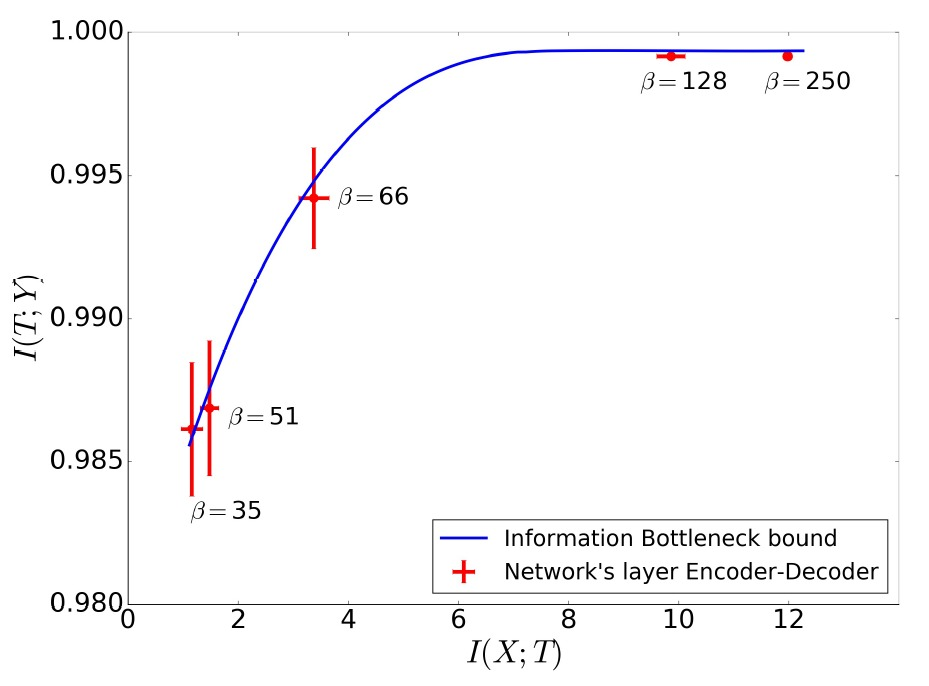
\includegraphics[width=\linewidth, height=\textheight, keepaspectratio]{figs/ib-curve.jpeg}
\label{fig:ib-curve}
\caption{The DNN layers converge to fixed-points of the IB equations. The error bars represent standard error measures with N=50. In each line there are 5 points for the different layers. For each point, $\beta$ is the optimal value that was found for the corresponding layer}
\end{figure}

\noindent \textbf{Information Plane} \\[0.15cm]
\indent One of the main contributions of the authors is to study the learning process of the model in the information plane (IP) introduced in \citep{Tishby2}. This visualizations show how mutual information $I(T;X)$ and $I(T;Y)$ evolve during the optimization process. Having randomly initialized layers, the deeper layers fail to preserve the information about the input at the beginning of the training (due to the Data Processing Inequality \citep{dpi}). We also observe that deeper layers have nearly no MI with the labels, which is expected. In the first phase of the learning process, the model fits to the data and tries to improve its predictions. In the second much slower phase, the mutual information measures move to the upper left direction, in other words layers lose information about their input while slightly increasing information about the labels.\\This phase is also called the compression or diffusion phase. The authors claim that the compression part of the training is responsible for reducing generalization error.\\

\noindent \textbf{Stochastic Gradient Descent} \\[0.15cm]
\indent In our opinion, the most interesting part of the paper is the explanation of how DNN achieve compression. The mean and variance of the norms of the gradients per layer are plotted in Fig.2. We can distinguish two parts (again): for the first 300 epochs, the gradients have a high norm and very small deviations. Then the variance starts becoming much more important than the norm of the gradients. Notice that these two time intervals are exactly corresponding to the two phases observed previously in the information plane. While the network is fitting the data, the loss is decreasing rapidly, it is thus expected to have large gradients with low variance. The more surprising result is why are noisy gradients responsible for compression? The authors explain that Stochastic Gradient Descent is equivalent to a Random Walk in the parameter space of the loss function. This Random Walk adds random noise to the weights, increasing the entropy of layers $T_i$ with respect to the inputs while still minimizing training error.  Having an increasing conditional entropy $H(X|T_i)$ causes a decreasing mutual information $I(X;T_i)$, because the input entropy $H(X)$ remains unchanged.\\

\begin{figure}[!htb]
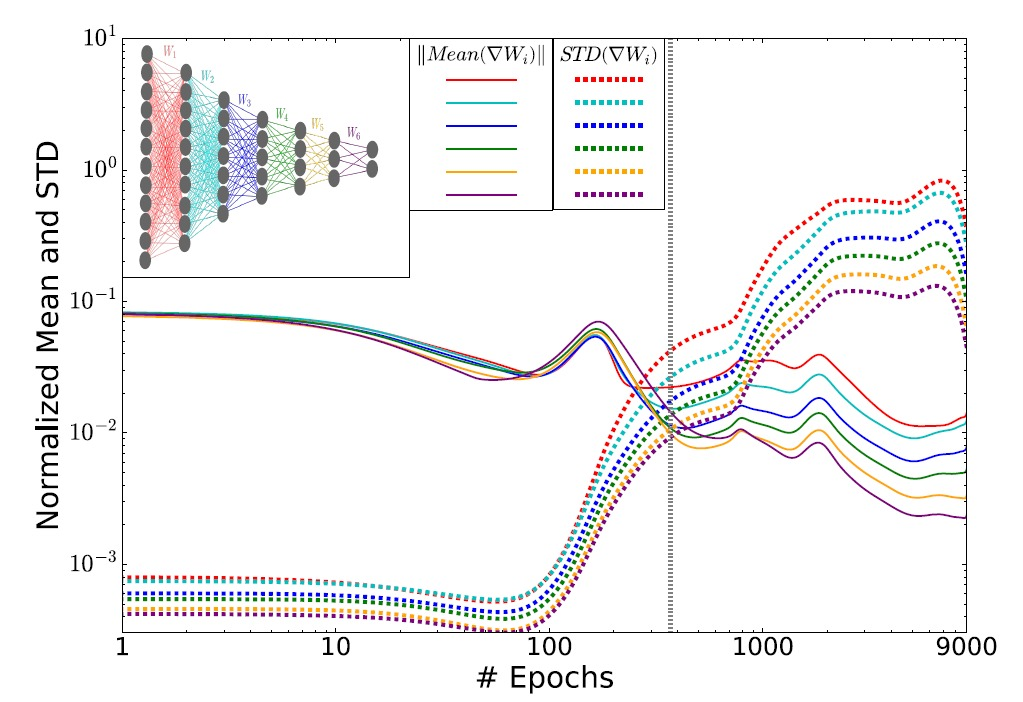
\includegraphics[width=\linewidth, height=\textheight, keepaspectratio]{figs/gradients.jpeg}
\label{fig:sgd}
\caption{The layers Stochastic Gradients distributions during the optimization process. The norm of the means and standard deviations of the weights gradients for each layer, as function of the number of training epochs (in log-log scale). }
\end{figure}


\noindent \textbf{Overfitting and Hidden Layers} \\[0.15cm]
\indent These new insights help us better understand two well-known phenomena in deep learning: \textit{overfitting} and \textit{deeper models make the model generalize faster}. \\
\indent \textit{Overfitting} can be analyzed in the information plane (see Fig.3). We observe that overfitting occurs mostly in the compression phase, i.e. overfitting can be seen as overcompression, the layers simplify the representation too much. \\

\indent \textit{The computational benefit of deeper NN} is according to the authors due to the fact that adding more hidden layers helps the compression go faster, thus generalizing faster. Previously, we saw that the SGD can be seen as a Random Walk, from the Focker-Planck equation \cite{fokker}, the quantity of entropy increase is deduced as 
\begin{equation}
\Delta H \propto log(D\tau)
\label{eq:propto}
\end{equation}
with $D$ a diffusion constant and $\tau$ the number of epochs. The number of epoch needed to make a compression $\Delta I_X$ grows exponentially as $\text{exp}(\Delta I_X / D)$. If we split the compression task between K hidden layers, each layer compresses $\Delta I^k_X$, with $\sum_k \Delta I^k_X = \Delta I_X$. The time needed for these K layers to achieve the same compression as one layer is $\sum_k \text{exp}(\Delta I^k_X/D)$. However the exponential of a sum is much larger than the sum of an exponential. This explains why compression is achieved faster when we make the network deeper.

\begin{figure*}[!htb]
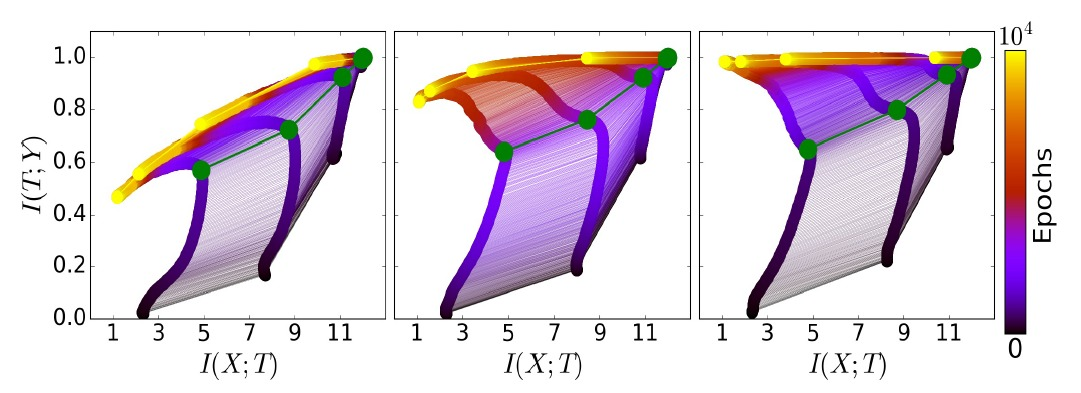
\includegraphics[width=\textwidth, height=\textheight, keepaspectratio]{figs/overfitting.jpeg}
\label{fig:overfitting}
\caption{The evolution of the layers with the training epochs in the information plane, for different training samples. On the left - 5\% of the data, middle - 45\% of the data, and right - 85\% of
the data. The colors indicate the number of training epochs with Stochastic Gradient Descent from 0 to 10000. The network architecture was fully connected layers, with widths:
input=12-10-8-6-4-2-1=output. The examples were generated by the spherical symmetric
rule described in the text. }
\end{figure*}

\section{Discussion}

A major drawback of the paper is that experiments where performed on a simple DNN with saturating activation functions. Saxe et al.\citep{saxe} showed that when using the very common ReLU function, the DNN yields no clear sign of compression. However Tishby claims the experiments of Saxe et al.\citep{saxe} are invalid because their methodology for estimating MI is not robust. This was indeed confirmed recently by Chelombiev et al.\cite{MI1}, they justified that a DNN using non-saturating functions, results in unbounded hidden activity. The level of noise brought by the binning process (see Section \ref{sec:background}) during the estimation becomes not consistent. To counter this undesired effect, Chelombiev et al.\cite{MI1} developed an adaptive estimator. Their findings showed in the information plane the fast fitting then slow compression pattern, even for a ReLU function.\\
\indent Another limitation of the paper is that it would have been easy to verify partially the conclusions on consequent datasets like ImageNet\cite{imagenet}. Indeed a common trick is to stop the training process once the validation error oscillates around its lowest point. The authors could have continued training for a long time and verify if the model does indeed generalize better, for example using adversarial examples.\\
\indent An important issue preventing the IB to be easily integrated in a DL setting is that mutual information estimation is computationally expensive in real-world machine learning problems. Possible solutions involve developing faster estimators \citep{MI1, MI2} or as suggested by Tishby in one of his talks, use the order of magnitude of the proportion between mean and variance of the gradients as a proxy for MI estimation. \\
\indent In \citep{vib} a very interesting relationship between Variational Auto-encoders (VAE) \citep{Kingma} and the Information Bottleneck was discovered. If we replace $I(T;Y)$ by $ H(Y)-H(Y|T)$, the IB optimization (\ref{eq:lagrange}) becomes 
\begin{equation}
\min_{p(t|x)} I(X;T) + \beta H(Y|T)
\label{eq:new-lagrange}
\end{equation}
Moreover,
\begin{equation}
H(Y|T) = \mathbb{E}_{p(x,y)} \left[\mathbb{E}_{p(t,X)}\left[-log(p(Y|T))\right]\right]
\end{equation}\vspace*{-0.1mm}
\begin{equation}
I(X|T) = \mathbb{E}_{p(x)} \left[\text{KL}(p(t|X) || p(t) \right]
\end{equation}
If those expressions are substituted in Eq.\ref{eq:new-lagrange}, the IB can be approximated by a loss function as,
$$
\mathcal{L} = \frac{1}{N} \sum_{i=1}^{N} \mathbb{E}_{p(t|x^{(i)})} \left[-log(p(y^{(i)}|t))\right] + \beta \, \text{KL}(p(t|x^{(i)}) || p(t))
$$
This equation is equivalent to the VAE loss in the special case when $\beta = 1$. It was shown that using a VAE with a hyperparameter $\beta > 1$ beats several state-of-the art results. This relationship, in our opinion conforts the justification of using MI as a tool to analyze or improve DL techniques. \\
\indent It is also worth noting that noise plays an important role in compression, and thus improving generalization. One could imagine using noise to improve existing optimization algorithms or even develop new ones.\\
\indent One last comment, is that all results of the IB applied to DL are valid only because we assume that a DNN can be modelled as a Markov Chain. The question is are we sure this is always true? For example, what happens if residual connections are used? 

% ==============================================================================

\bibliographystyle{unsrt}
\bibliography{bibliography.bib}

\end{document}